%!TEX root = presentazionelancia.tex
\section{Workload \& Performance}
\begin{frame}[c]\frametitle{Workload}
\centering
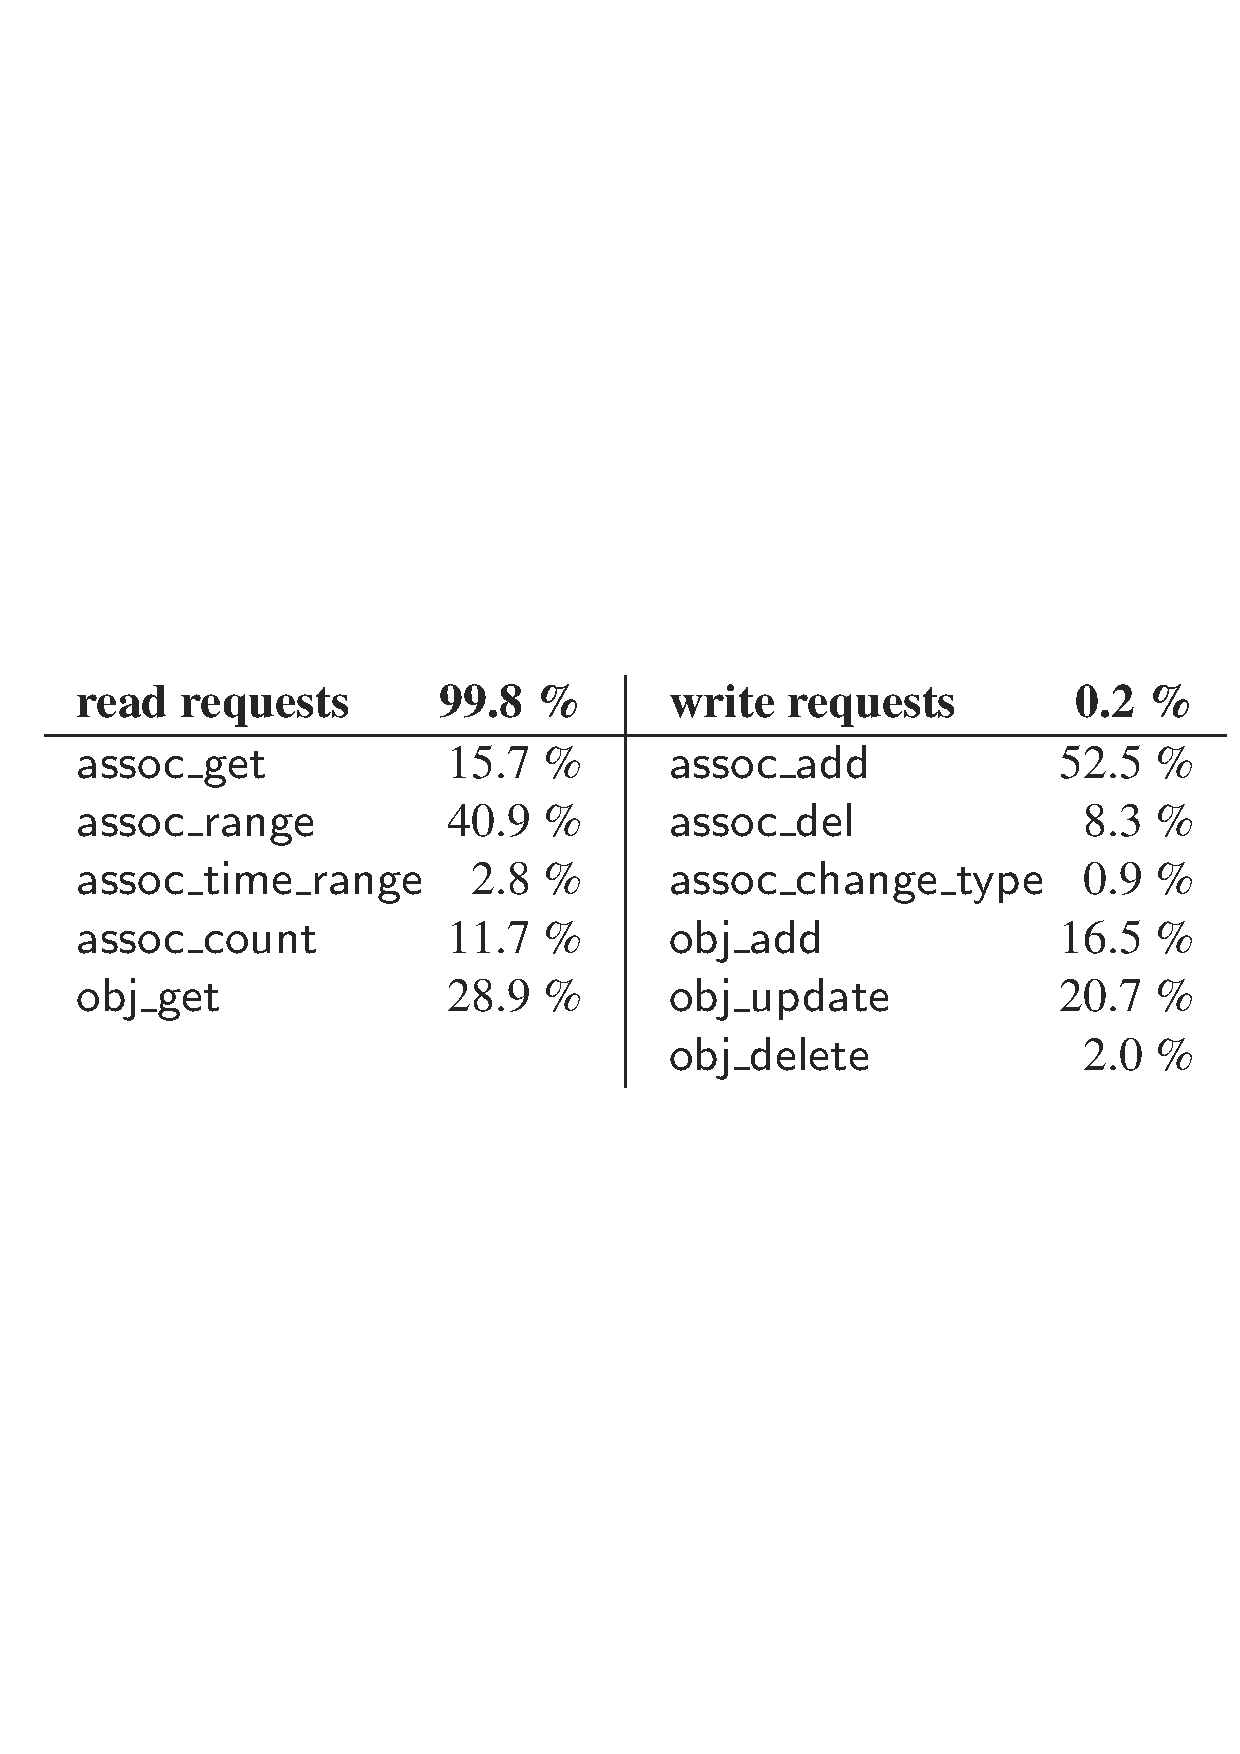
\includegraphics[width=\textwidth]{figs/table3.pdf} 

Frequencies for client request



\end{frame}

\begin{frame}[c]\frametitle{Availability}
Under real workload, over a period of 90 days, the \textbf{fraction of failed TAO queries} is:
\begin{center}
	\huge $4.9 \times 10^{-6}$
\end{center}

\end{frame}
\begin{frame}[c]\frametitle{Followers Capacity}
	\centering
    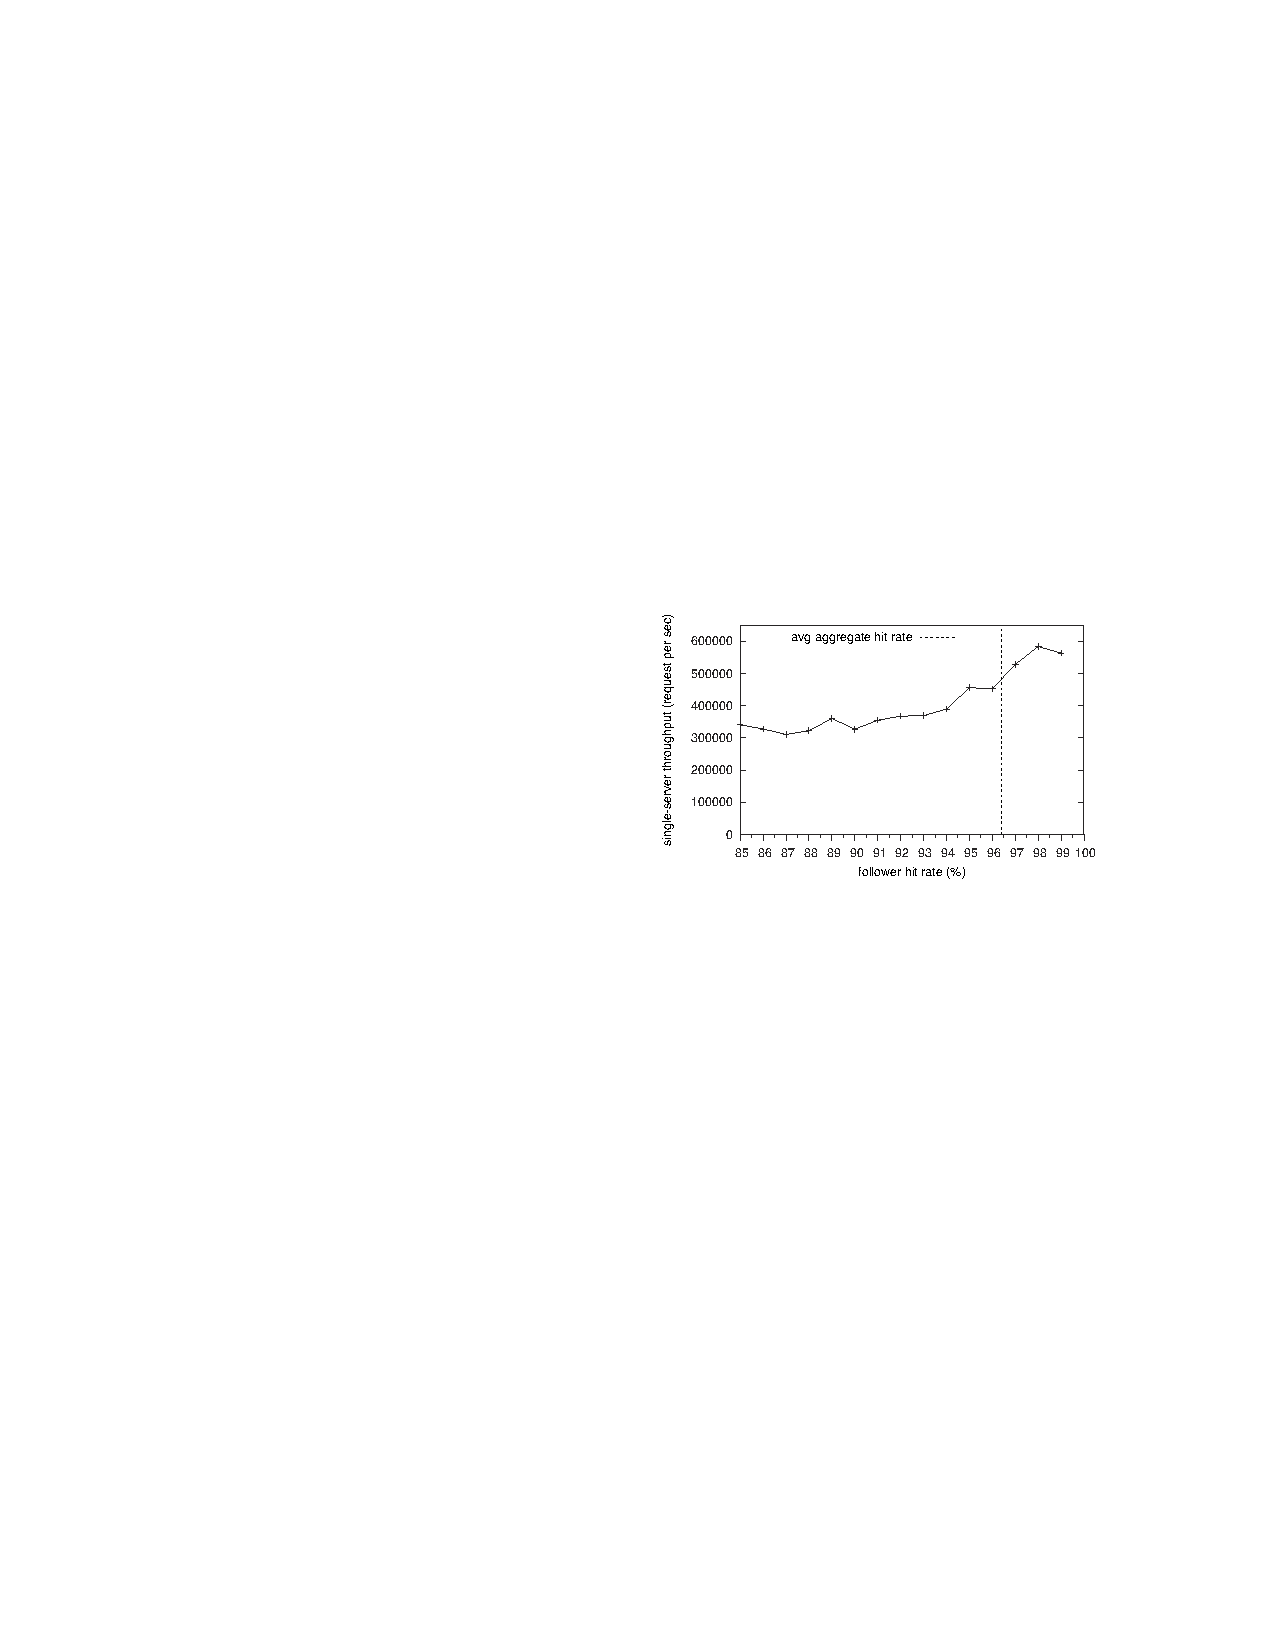
\includegraphics[width=\textwidth]{figs/followercapacity.pdf}
\end{frame}

\begin{frame}[c]\frametitle{Hit Rates and latency}
\centering
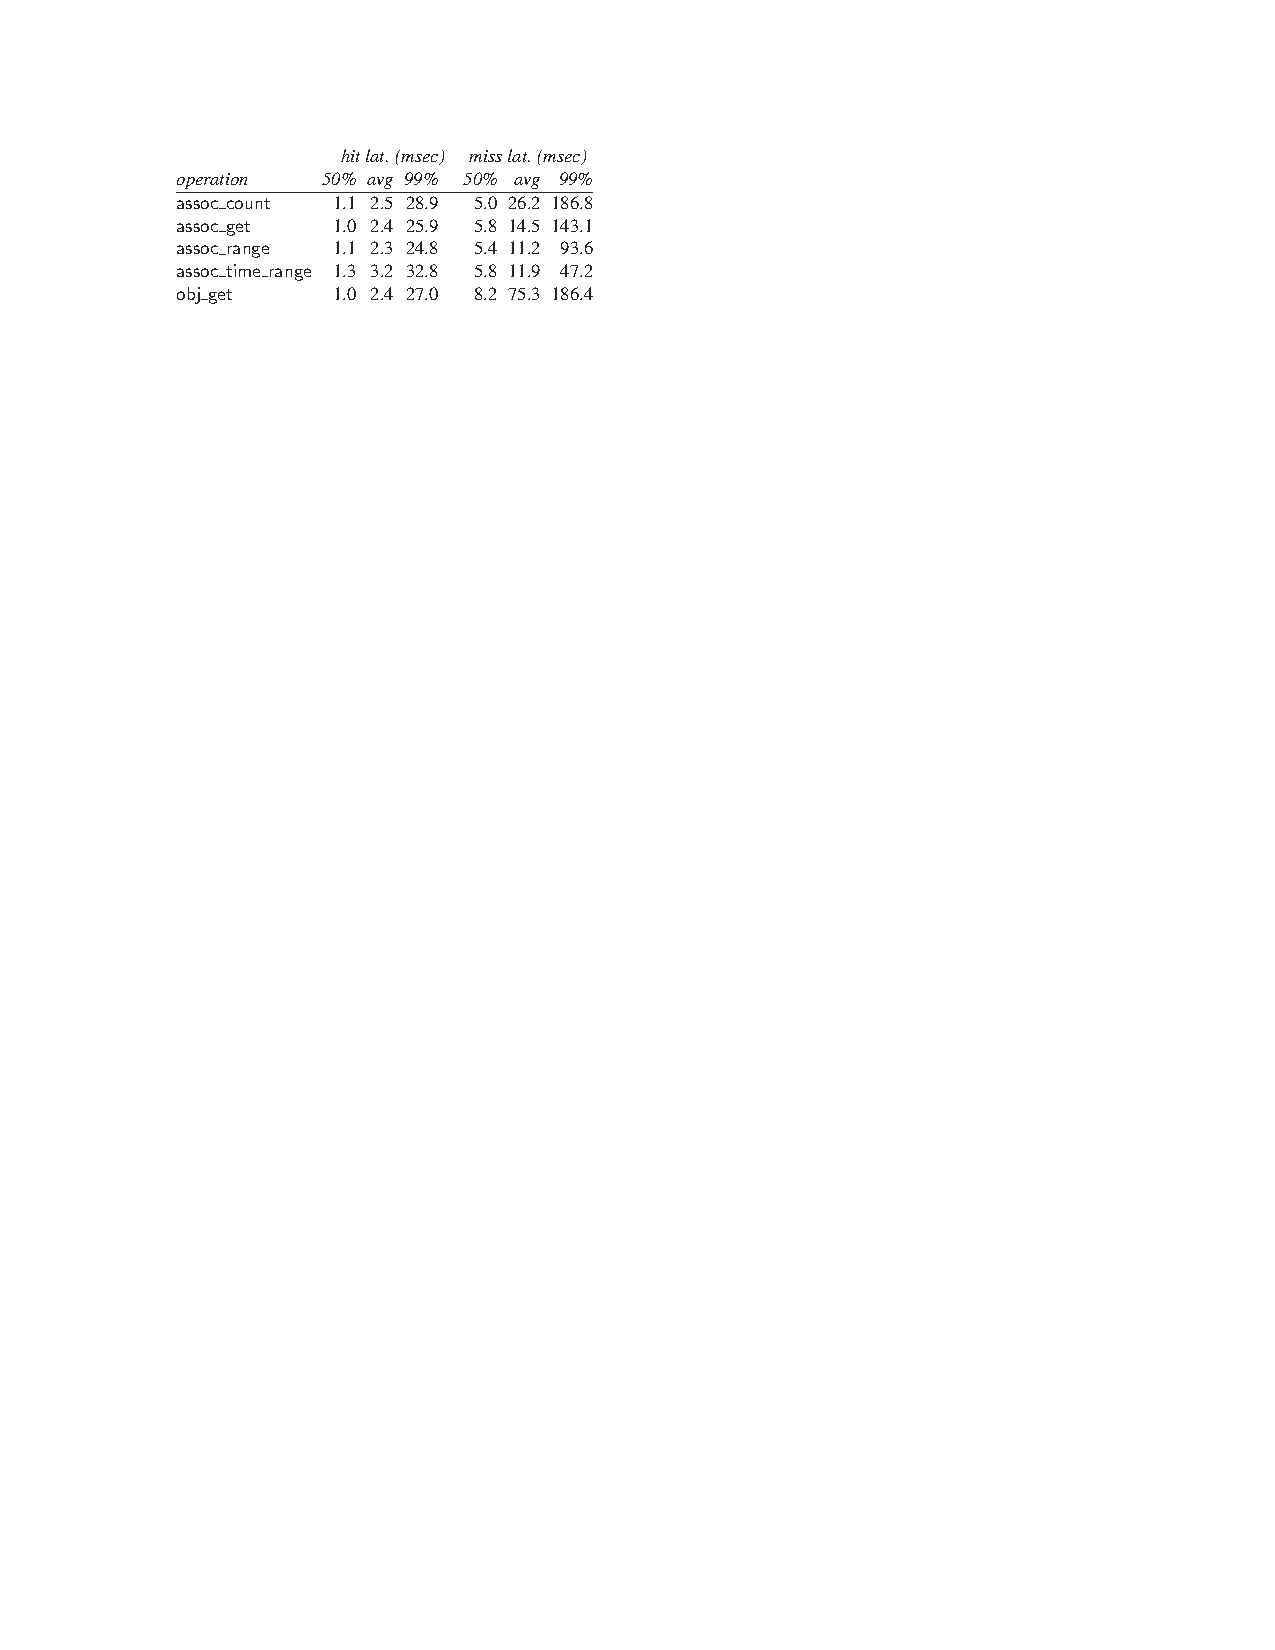
\includegraphics[width=\textwidth]{figs/table8.pdf} 

\end{frame}

\begin{frame}[c]\frametitle{Write Latency}
   	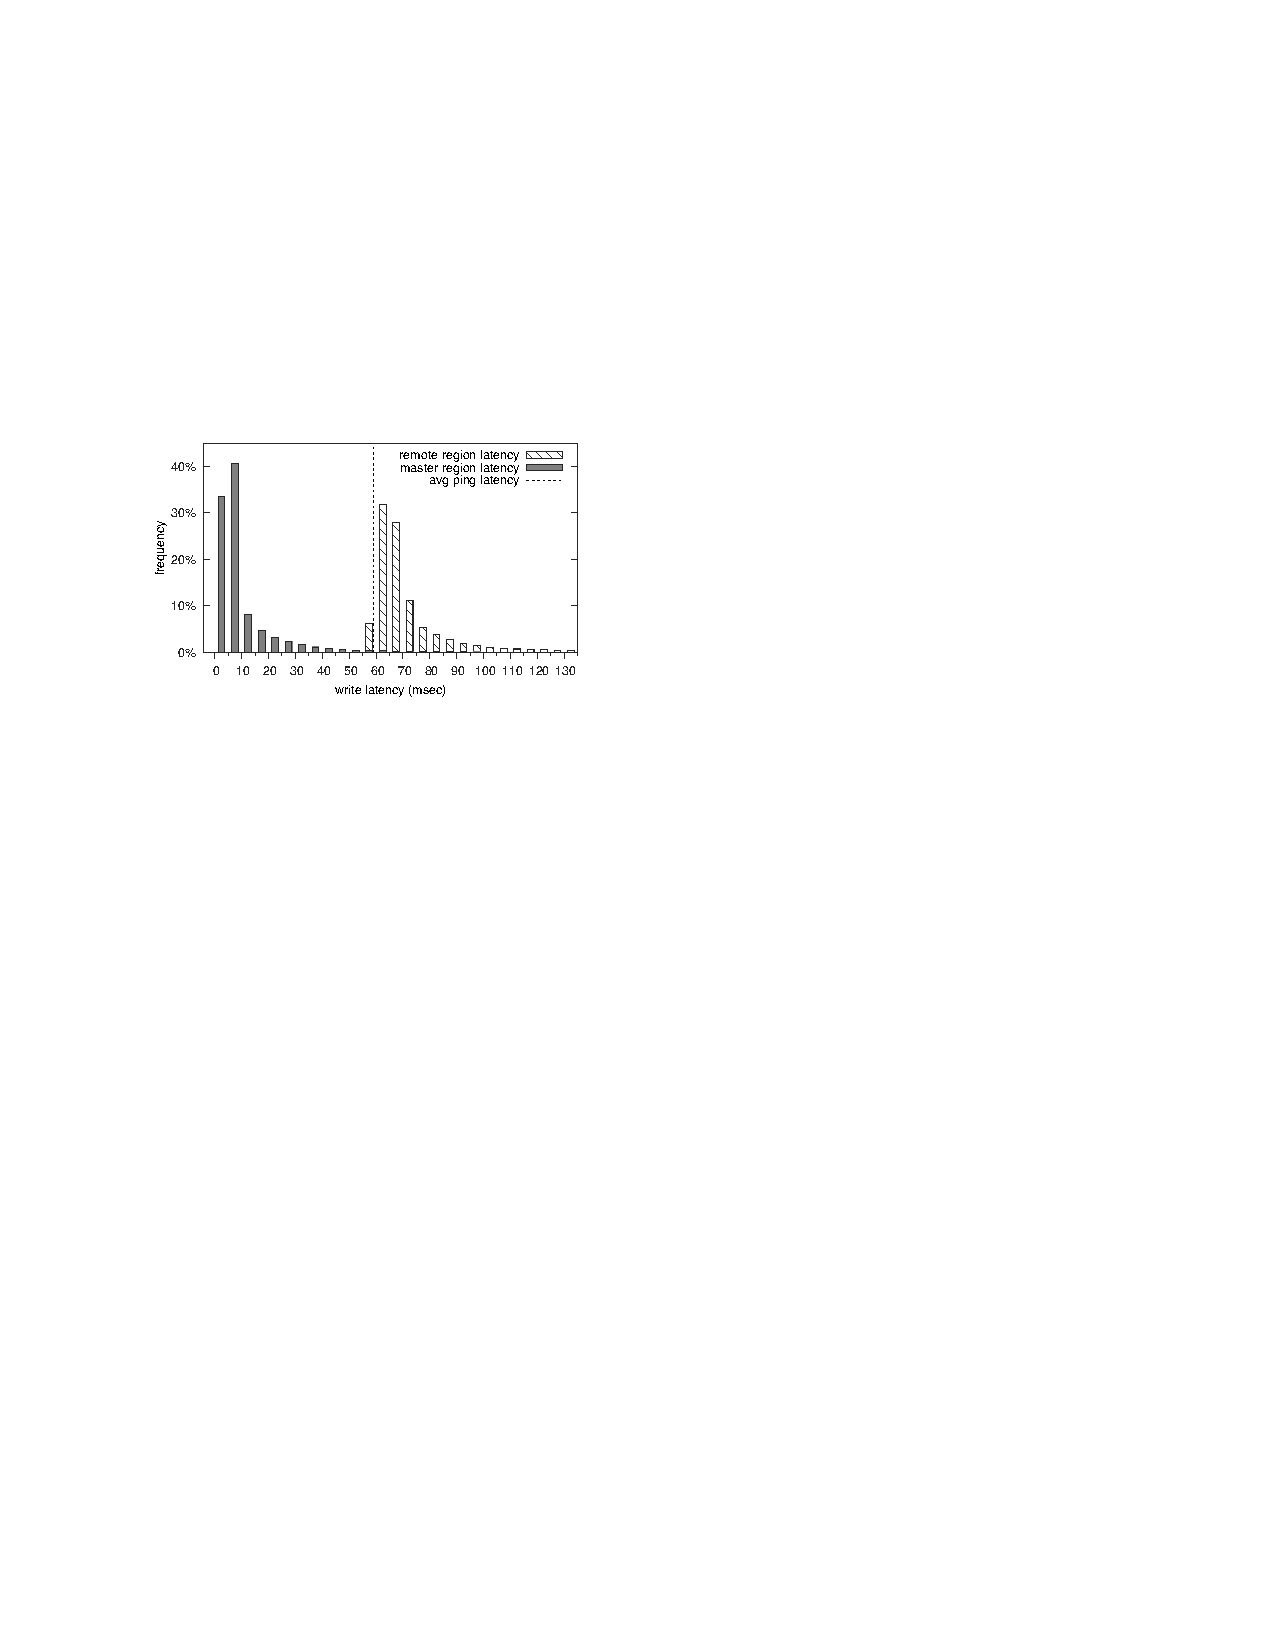
\includegraphics[width=\textwidth]{figs/writes.pdf}
\end{frame}


\begin{frame}[c]\frametitle{Summarizing}
\begin{description}
	\item[Read latency] \hfill\\
	\begin{itemize}
		\item Separate cache from database
		\item Graph aware cache
	\end{itemize}
	\item[Efficiency at scale] \hfill\\
	\begin{itemize}
		\item Subdividing Data Centers
	\end{itemize}
	\item[Write timeliness]\hfill\\
	\begin{itemize}
		\item Write trough cache
		\item Async replication
	\end{itemize}
	\item[Read availability]\hfill\\
	\begin{itemize}
		\item Multiple data sources
	\end{itemize}
\end{description}


\end{frame}